\section{Task Overview}
The application is split into 4 main FreeRTOS tasks with specific priorities: 
\begin{table}[h!]
    \centering
    \begin{tabular}{|c|c|p{8cm}|} % Adjust width (8cm) as needed
        \hline
        \textbf{Task Name} & \textbf{Priority} & \textbf{Role} \\\hline
        CHECK/SAFETY & High & Monitors health data. Checks for actuator overcurrents and IC overheating. It can trigger interrupt routines to enter safe states (e.g., reducing PWM duty cycle). \\\hline
        CONTROL & Normal & The core logic. Executes the attitude control algorithm (PD controller). It handles 3 OpModes: IDLE (0), CONTROL (1), and TEST/POLARITY (2). \\\hline
        OBC-COMM & Normal & Handles communication with the On-Board Computer (OBC). Receives target data and sends telemetry. \\\hline
        IMU & Normal & Samples angular speed and magnetic field from the IMU and sends data to Control and OBC tasks. \\\hline
    \end{tabular}
    \caption{Task overview with priorities and roles}
    \label{tab:tasks}
\end{table}

\subsection{CHECK/SAFETY Task}
The CHECK/SAFETY Task performs the following operations. 
\newline\\
\twominipages{.5}{.45}{
    \subsubsection{Actuator Overcurrent}
The task monitors all the actuators current (3 magnetorquers), ensuring that enough current is driven to every driver. 
\subsubsection{IC Overheating}
The task monitors the temperature of critical ICs, as the CPU and actuators. If the CPU excees a critical temperature the system MUST be put in a temporary IDLE/SAFE state. If actuators overheat, the amount of current is reduced by modifying the Duty Cycle of the PWM signal for the specific actuator. 
\newline\\
The device enters a safe state whenever a temperature overcome or an overcurrent happen. This event MUST be avoided to not endanger the system during the mission. 
}{
    \centering
    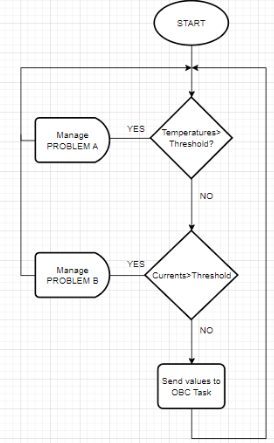
\includegraphics[width=0.7\linewidth]{assets/images/03/check_flow.png}
    \captioninminip{CHECK Task Flowchart}
} 
\newline\\
\cimage{assets/images/03/problemA.png}{10}{Problem A Flowchart}
\newline
\section{Scheduling Logic}

\section{Synchronization Strategy}